\chapter{Predicting optimal Spark settings in standalone mode}

\emph{Abtsract} What are the optimal parameter settings for a long running, standalone mode, Spark-based stateless process? The chapter investigates the effects of four different Spark parameters, and compares the application's behaviour in two different servers. Two important lessons learned from this experiment are: i) allocating more resources (e.g. memory, CPU) does not necessary imply better performance of the process, ii) in an environment with limited and shared resources instead of maximising the performance one should rather tune the system to be `good enough' in terms of performance and at the same time is respectful with other running processes. To discover the optimal settings, it is suggested to pick a small sample that shares important features with the full dataset, and measure performance of the process against different Spark parameter settings. The settings to check are: the number of cores, memory allocation, compression of the source files, and reading data stored on different file systems (if they are available). As a source of ground truth, Spark log, Spark event log, or measuring points inside the application, can be used.

%\keywords{Apache Spark \and performance metrics \and metadata quality \and Europeana.}

\section{Introduction}
Measuring the quality of cultural heritage metadata is a task which has two important features. First, in Digital Humanities (DH) context the size of source data (catalogues of libraries, archives, and museums -- commonly abbreviated as LAM; or aggregated catalogues and datasets such as Europeana\footnote{\url{https://europeana.eu}}, Wikidata\footnote{\url{https://wikidata.org}} or Archives Portal Europe\footnote{\url{http://www.archivesportaleurope.net/}}) could be regarded as Big Data. Big Data is a relative concept, usually referring to data larger than can be processed by traditional methods within the available infrastructure of a LAM organisation. DH and cultural heritage contexts have not traditionally been equipped with high performance computing tools, so the volume of Big Data managed in these contexts has been generally smaller than, for example, in the fields of astrophysics or medicine. On the other hand, the variety of data in DH and cultural heritage contexts is large. Second, even after a decade of research in metadata quality (\cite{zotero-bibliography}), the LAM community has not yet reach a clear consensus on the exact meaning of `quality' -- however different quality dimensions and metrics have been established

Current research (Measuring Metadata Quality) is still experimental, and based (to an extent) on trial and error workflow, in which metrics are selected from the literature  (or new metrics are invented); their measurements are implemented and tried on the (meta)data; and metadata experts evaluate the result and suggest changes on the measurement. A consequence of this research cycle is that it necessitates the execution of multiple long running measurements of the same Big Data set. It takes considerable time, and requires a significant allocation of computer resources (memory, CPU, disk capacity), with a tendency to block other tasks running concurrently on the same computer. Apache Spark\footnote{\url{http://spark.apache.org/}} among other tools, decreases the duration of this research cycle by letting the existing process run in parallel fashion. While Spark could be run in a cluster, clusters are rarely available to DH/LAM organizations, where a more typical use is to run Spark in `standalone mode' utilising the multicore architecture of a single machine and simplifying the writing of multi-threaded software code. This chapter suggests easy preliminary measurements for a Spark-based process to identify its optimal settings in each context. Another aim of this chapter to fulfil a gap in the literature concerning Spark’s usage and performance in standalone contexts, as commercial and scientific conference presentations concerning Spark’s performance concentrate upon its work in clustered environments.

\section{Measuring completeness of Europeana records}

Europeana is a digital platform of the European cultural heritage, which aggregates catalogue records from European libraries, archives, museums, and other cultural organisations (called data providers). This experimental research uses a snapshot of Europeana records created during 2018 August containing approximately 62 million records. Each record are in Europeana Data Model (EDM)\footnote{\url{https://pro.europeana.eu/resources/standardization-tools/edm-documentation}} metadata schema, which has the several parts or `entities': a descriptive metadata part (`proxy'), and optional contextual entities that describe the agents, concepts, places and time spans mentioned in the proxy. Moreover Europeana not only aggregates these records, it enhances them as well. With the help of semantic web technologies and linked open data, Europeana attempts to detect entities in the data provider's proxy, and to save them as additional contextual entities.

The snapshot of Europeana’s data used in this research is stored in a MongoDB database. Accessing MongoDB from Spark has limitations as reading from MongoDB is a time-consuming process, and Spark's Mongo connector does not support a specific reference type which is heavily used in the database. As such, the author chose to export the data in text files in which every line is an individual, normalised record.\footnote{Here, `normalisation' refers to the record packaging together the proxies and all linked contextual entities, instead of merely keeping references to them.} This process was built upon Spark's Mongo connector, enhanced with some extra API calls\footnote{\url{https://github.com/pkiraly/europeana-qa-spark}}. Spark's Mongo connector partitions the database in order to run the processing tasks (reading and and exporting records to text files) in parallel. At the end of the process 1740 files -- each with 35.6 thousand records -- were created. The size of the files varies, averaging 0.47GB in size; the bulk of files are between 0.23 GB and 0.9 GB.

This preparation phase was followed by a record-level-measuring process using Spark's Java API. Within the broader research project (Measuring Metadata Quality) the author conducted multiple measurements. For this experiment, one of them, the \emph{completeness measurement} was selected. The completeness measurement takes a JSON string and checks every field in the schema that is available in that record, and returns an integer (zero or more) denoting the number of available field instances. The result is serialised as a CSV formatted string containing record identifiers, some metadata (the identifiers of sources of the records), and the cardinalities of the fields. Spark takes care of reading the input, writing the output, and distribution of the processing over the available CPUs. The part of the process that interacts with Spark is provided below in Listing \ref{code:spark_api_usage}. The next step is the statistical analyses of this CSV file. This produces, in turn, a set of CSV files with statistical description of the whole collection and its 20 thousand subcollections (that is, records harvested in the same dataset, created by the same data provider, aggregated by the same provider, derived from particular countries, or written in the same language -- or the combination of these), an their visualisation on a web based user interface.

The standalone Spark process is a minimalistic use of Spark API's capabilities -- above its mandatory input and output calls only one extra method is used: map(). It is important to note that Spark API is similar to SQL queries: it is a high level API, and its engine optimises it and creates a low level implementation. When the Spark process is started, it analyses the input to calculate the number of `tasks' it needs to complete. Each task takes an input, runs the code, and saves the output. Outside of these tasks Spark runs a monitoring web server, which is started before reading the first file, and shut down after producing the last output. Spark also runs some file managing processes in the background when merging and renaming output files. The final output will be a set of files, which need to be merged into a single file outside of the standalone Spark process.

\begin{lstlisting}[
  % one can adjust spacing here if required
  % aboveskip=2.5\baselineskip,
  % belowskip=-.8\baselineskip,
  caption={The part of Java client code which interacts with Spark API},
  label=code:spark_api_usage,
  language=Java,
  float]
// initialize Spark
SparkConf conf = new SparkConf().setAppName("CompletenessCount");
JavaSparkContext context = new JavaSparkContext(conf);

// initialize the processing class
final EdmCalculatorFacade facade = ... 

// read input file
JavaRDD<String> inputFile = context.textFile(parameters.getInputFileName());

// definition of a method which process a lines
Function<String, String> baseCounts = new Function<String, String>() {
  @Override
  public String call(String jsonString) throws Exception {
    String result = "";
    try {
      result = facade.measure(jsonString);
    } catch (InvalidJsonException e) {
      // error reporting
    }
    return result;
  }
};

// processing every lines of input files
JavaRDD<String> baseCountsRDD = inputFile.map(baseCounts);

// save result
baseCountsRDD.saveAsTextFile(parameters.getOutputFileName());
\end{lstlisting}

\section{Tuning Spark and measuring performance}

There are several settings in standalone Spark process which are deserving of further experimentation:
\begin{itemize}
 \setlength{\parskip}{0pt}
 \setlength{\itemsep}{0pt plus 1pt}
 \item number of cores (CPUs) of the processing computer;
 \item memory allocation
 \item for file inputs:
 \begin{itemize}
  \setlength{\parskip}{0pt}
  \setlength{\itemsep}{0pt plus 1pt}
  \item whether they are stored in the operating-system's file system, or in a Hadoop File System
  \item whether they are compressed of not
 \end{itemize}
\end{itemize}

In the experiment the author ran the same measurement on two different machines using two input sets. The first input set is the full corpus, while the second input set contains only ten files. The average size of these files are smaller than the average size of files in the whole collection (mean is 0.3 GB, while it is 0.47 GB for the full set). The first machine (`europeana') has a CPU 2.4 times faster than the second one (`roedel'). `Europeana' has eight cores, `roedel' has 16 cores. The data and the processing code were identical, and both machines used Spark version 2.4.0.

The numbers measured are recorded in different sources. Spark log provides information about `stage' and `job' duration. In the Spark processing hierarchy the process might be split into multiple jobs, each having multiple stages; in this experiment there is only one job with a single stage. The process is launched by a bash script, which also measures the overall duration. Spark has a special event log (see later), which provides other important metrics, such as executors' run-time and CPU-time. Finally the author put a time counter into the client source code, to record how much time the map() function takes to complete the process (see Listing \ref{code:spark_accumulator}). Bash scripts read these information, and the charts were created with R.\footnote{The source files of the experiment are available at \url{https://github.com/pkiraly/euro-par}.}

\begin{lstlisting}[
  % one can adjust spacing here if required
  % aboveskip=2.5\baselineskip,
  % belowskip=-.8\baselineskip,
  caption={Use of Spark accumulator to measure duration},
  label=code:spark_accumulator,
  language=Java,
  float]
// accomulators are special, thread-safe, distributed Spark variables
LongAccumulator accum = context.sc().longAccumulator();

...
Function<String, String> baseCounts = new Function<String, String>() {
  @Override
  public String call(String jsonString) throws Exception {
    long start = System.nanoTime();
    ...
	accum.add(System.nanoTime() - start);
    return result;
  }
};
...
logger.info(formatDurationInfo(accum));
accum.reset();
\end{lstlisting}

\subsection{Number of cores and compression}

In next experiment, the effect of the number of cores used, and whether the files were compressed, has been measured. The appropriate parameters are listed in Listing \ref{code:spark_cores}. The results (the processing time per record under given number of cores) are displayed in Fig. \ref{figure:small-and-full-measurements-two-servers}. A number of conclusions could be drawn from the chart.

\begin{lstlisting}[
  % one can adjust spacing here if required
  % aboveskip=2.5\baselineskip,
  % belowskip=-.8\baselineskip,
  caption={Spark settings for number of cores and input specification},
  label=code:spark_cores,
  language=Bash,
  float]
spark-submit --master local[<number-of-cores>] --inputFileName file:///...
\end{lstlisting}

\begin{figure}
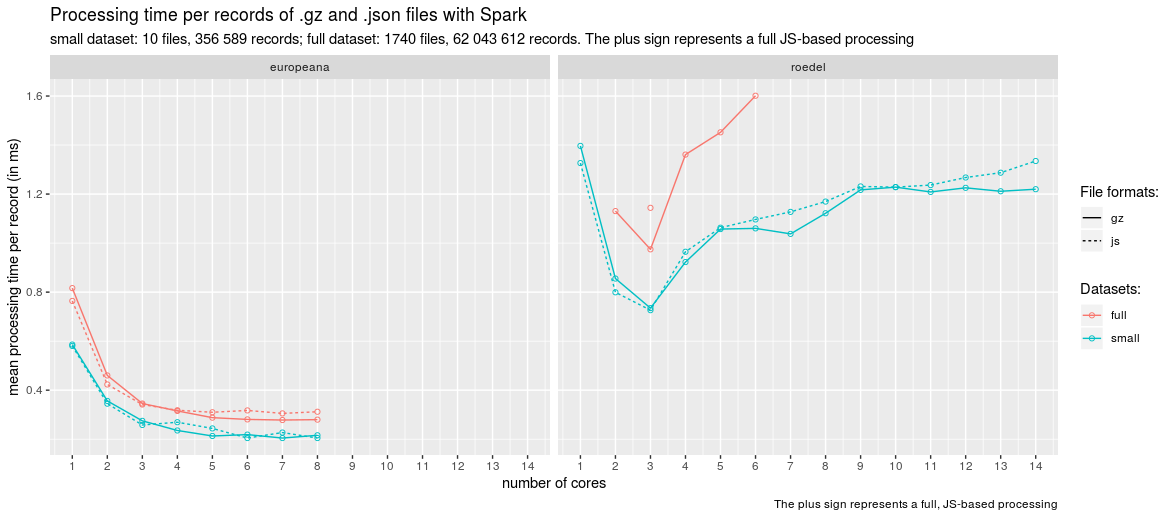
\includegraphics[width=\textwidth]{images/chapter06/small-and-full-measurements-two-servers.png}
\caption{Processing time per records with different settings}
\label{figure:small-and-full-measurements-two-servers}
\end{figure}

1) The per record processing times for the small set is faster. It is not surprising given, that processing time depends on the complexity of the record structure which correlates with the size of the record. It is more important that the shape of the small set and the full set are close to each other; correspondingly, running a small set for this kind of application might predict the running of the full set. It is important that the processing function -- that is, `measure()' -- is stateless, ensuring the incorporating classes do not collect data (unless in exceptional cases), and the measurement undertaken does not depend upon previous records. Not all Spark client code works this way: the prediction holds only for stateless ones.

2) Gzip compressed files are usually slightly faster than uncompressed files. Processing compressed files has two side effects. First, uncompressed files are partitioned, and (as we saw above) each partition is paired with a distinct task with its own overhead. Second, decompression also has its own overhead. The evident advantage of using compressed files is sparing of disk space.\footnote{Since the full process took more than one day on `roedel' machine which exceeded the author's limited machine time, the fastest predictably setting was run on the uncompressed files.}

3) The shape of lines on the two machines are significantly different. On `euroepana', as more cores are engaged performance continually increases until seven cores, however after a given number of cores (3-4) the improvement is not significant. To determine the optimal settings for the number of cores is not easy here, because there is no clearly identifiable optimal core number. There are two discernible factors at play: first, the examined speed might be already `good enough'; second, while using more cores does slightly improve the performance of the current process, it takes resources away from other processes running on the same system, which is an impolite behaviour. On `roedel' the situation is radically different; it has a clear peak at 3 cores. The reason is that the system throughput -- that is, the combination of CPU, memory and I/O operation speed and other factors -- has a maximum. If more parallel processes are running, some processes will consume and lock all available resources thus creating a bottleneck because others will wait for moments until the locked resources have been released. To detect the actual bottleneck is not easy; some techniques for this task are discussed below.

\subsection{Memory allocation}

The next setting tested was the amount of allocated memory. The process was run on the small, compressed set using different number of cores and allocating 1, 2, 3, and 4 GB memory for both Spark driver (the central controller) and executors (the parts which execute client code). The Spark settings are available in Listing \ref{code:spark-memory}.

\begin{lstlisting}[
  % one can adjust spacing here if required
  % aboveskip=2.5\baselineskip,
  % belowskip=-.8\baselineskip,
  caption={Spark's memory allocation options},
  label=code:spark-memory,
  language=Bash,
  float]
spark-submit --driver-memory <memory> --executor-memory <memory> ...
\end{lstlisting}

\begin{figure}
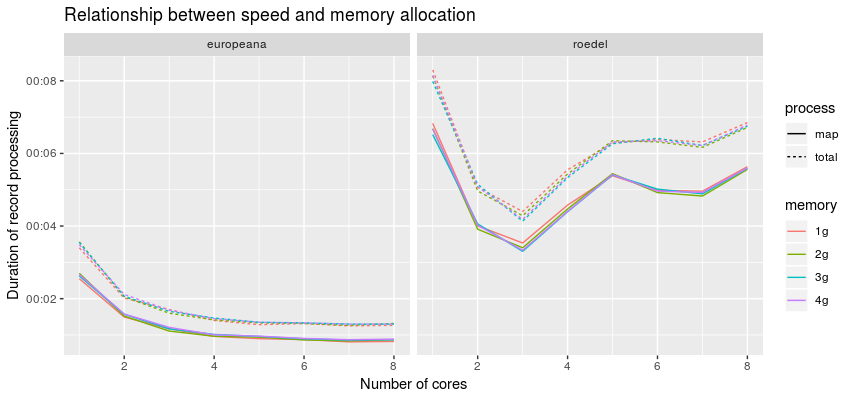
\includegraphics[width=\textwidth]{images/chapter06/memory-allocation-details.png}
\caption{Relationship between speed and memory allocation.}
\label{figure:memory-allocation-details}
\end{figure}

Fig. \ref{figure:memory-allocation-details} shows the result of different memory allocations. Succinctly, differences in allocated memory do not produce any clear effect. This is not a surprise, as the application is virtually stateless. If it were to accumulate large (or lots of) variables in memory -- which happens in several Spark SQL or Spark ML based applications -- we would see a significantly different graph. The conclusion is that it is not worth allocating more memory than the default for this application: which is 1 GB for the current Spark version.

\subsection{HDFS or normal FS?}

While Spark works well with Hadoop Distributed File System (HDFS)\footnote{\url{http://hadoop.apache.org/docs/current/hadoop-project-dist/hadoop-hdfs/HdfsDesign.html}}, this chapter questions whether Spark performs better in a standalone setup, where HDFS runs on a single machine, and is not distributed over nodes? The Spark settings is available in Listing \ref{code:hdfs}. The result is shown in Fig. \ref{figure:hdfs-vs-fs}.

\begin{lstlisting}[
  % one can adjust spacing here if required
  % aboveskip=2.5\baselineskip,
  % belowskip=-.8\baselineskip,
  caption={Reading from HDFS},
  label=code:hdfs,
  language=Bash,
  float]
spark-submit --inputFileName hdfs://localhost:9000/europeana/*.gz ...
\end{lstlisting}


\begin{figure}
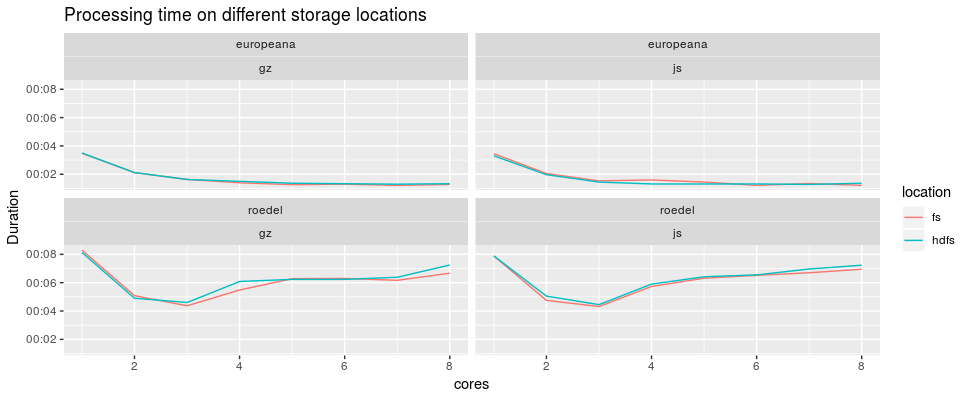
\includegraphics[width=\textwidth]{images/chapter06/hdfs-vs-fs.png}
\caption{Processing time on different storage locations}
\label{figure:hdfs-vs-fs}
\end{figure}

In most cases, the results are slightly better for operating system's file system, but not always, and usually the difference between the results is small. The question of whether it is worth to use HDFS or not depends on the speed gain and the cost of the setup of HDFS. The experiment shows there is little advantage in storing files in HDFS in these two test systems.

\section{Event log and history server -- to measure performance}

It was mentioned earlier that Spark launches a monitoring web service (unless it is disabled), that provides useful information about the running process. Although he application is shut down when the process ends, Spark provides a useful tool to keep historical information. To enable this tool requires the setting up a directory which stores the events (and their metrics). This history server is similar to the monitoring server, yet it processes data from the saved event log and not from the live process (as per the monitoring service).  As the event log is a simple text file containing JSON formatted lines, it is possible to move the event log and display its content on a different machine.\footnote{The event log file name consists of the master name and the timestamp of the start (such as `local-1550822115584'). This name is also used as an identifier inside the file. If required for use in another machine, file name should be changed, and its occurrences should be also changed inside the file content (e.g. in this experiment the author used names such as `europeana-c4', where `europeana' reflected to the machine name, while `c4' stands for experiment run with 4 cores setting).} It is important to note that the web interface does not show all the information from the event log. The history server provides an API, enabling data to be programmatically read from it.

\begin{lstlisting}[
  % one can adjust spacing here if required
  % aboveskip=2.5\baselineskip,
  % belowskip=-.8\baselineskip,
  caption={Spark history server setting and launch},
  label=code:history-server,
  language=Bash,
  float]
> cd $SPARK_HOME
> more conf/spark-defaults.conf
...
spark.eventLog.enabled         true
spark.eventLog.dir             file:/path/to/spark-event-log
spark.history.fs.logDirectory  file:/path/to/spark-event-log
> sbin/start-history-server.sh
\end{lstlisting}

\begin{figure}
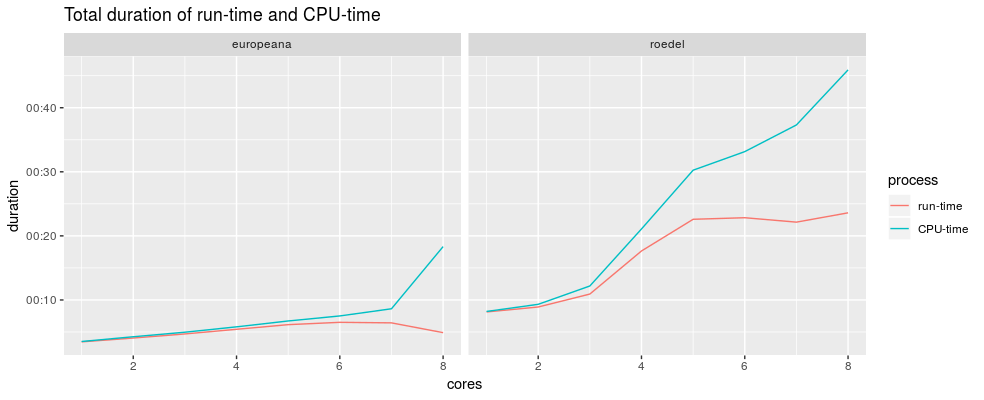
\includegraphics[width=\textwidth]{images/chapter06/runtime-vs-cputime-absolute.png}
\caption{Processing time on different storage locations}
\label{figure:runtime-vs-cputime-absolute}
\end{figure}

The most important information for this experiment are `executorRunTime' and `executorCpuTime' variables. According to Spark API documentation \cite{spark-taskmetrics} `executorRunTime' is the ``time the executor spends actually running the task (including fetching shuffle data)'', while `executorCpuTime' is the ``CPU Time the executor spends actually running the task (including fetching shuffle data) in nanoseconds''. Since the experiment process did not have shuffle steps, it can be supposed that most of the time happens inside the map() function. According to \cite{canali2017} the difference between run-time and CPU-time is the time the CPU waits for the memory. Fig. \ref{figure:runtime-vs-cputime-absolute} reveals that that the time spent on the map() function grows increasingly larger in both machines as the number of cores utilised are increased. It is natural, because individual processes will increasingly compete for resources. The two machines used in this experiment behave differently due to the increases in difference between times.

\begin{figure}
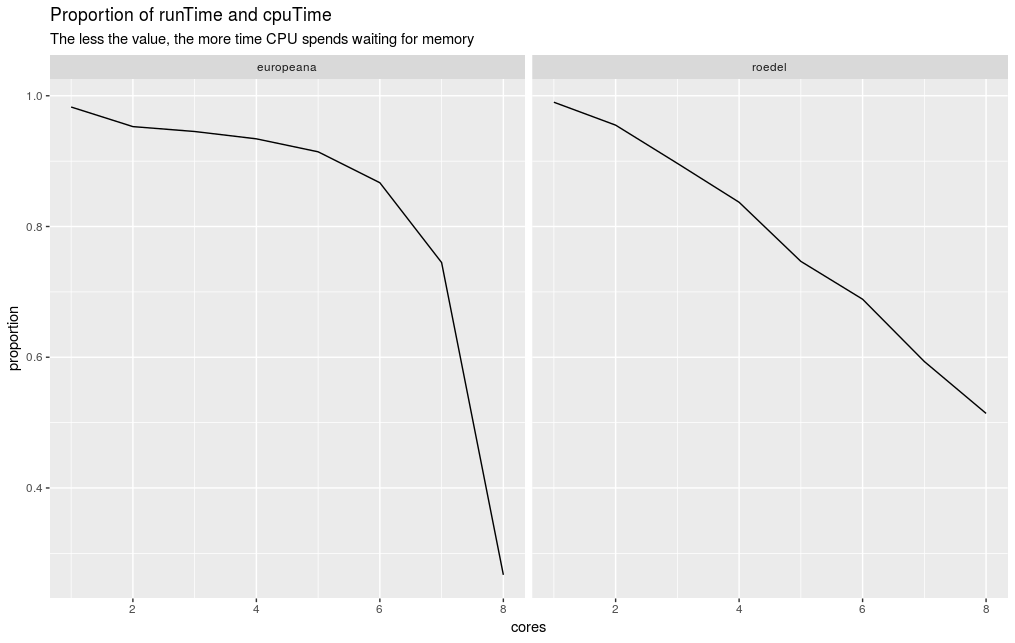
\includegraphics[width=\textwidth]{images/chapter06/runtime-vs-cputime.png}
\caption{Proportion of run-time and CPU-time. The larger the distance, the more time CPU is waiting.}
\label{figure:runtime-vs-cputime}
\end{figure}

If the time consumption were displayed differently, highlighting the relative numbers (i.e. the proportion of run-time and CPU-time in Fig. \ref{figure:runtime-vs-cputime}), an interesting pattern can be observed. While in `europeana' the degradation is moderated up until the utilisation of 6 cores, and from then on is progressive, on `roedel' the degradation is linear. This means that the CPU spends a lot of time waiting, including when performing well utilising only a small number of cores.

\begin{figure}
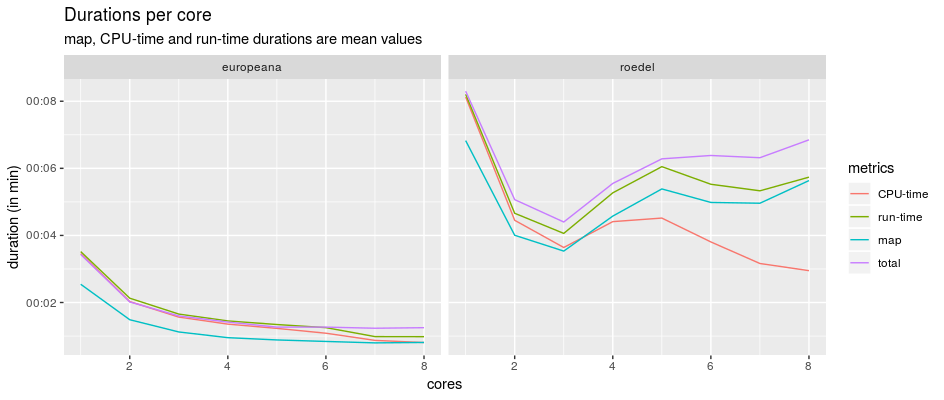
\includegraphics[width=\textwidth]{images/chapter06/all-durations.png}
\caption{Duration of different components per CPU.}
\label{figure:all-durations}
\end{figure}

In Figure \ref{figure:all-durations} run-time and CPU-time are displayed alongside the duration of the map method and total processing time. Figure \ref{figure:all-durations} reveals the reason of the performance peak: the quickest performance happens before the duration of the map method exceeds the CPU-time. It is not clear exactly what other processes are involved in the task, yet it is clear, that the CPU is undertaking other processes concurrently as the crossing CPU-time is larger then the duration of the map method. When the duration of the map method gets bigger than the CPU-time, it is clear that map() function -- and the other confounded processes -- has to wait for free memory. Notably, this crossing occured on `europeana' between 7 and 8 cores, and on `roedel' between 3 and 4 cores. It is also interesting that at 8 cores on `roedel' the map-time almost reaches run-time, and almost half of its time is spent waiting.

One last note about the hidden processes. As mentioned earlier, Spark optimises its code, and this code is not the high level API which runs in the Java Virtual Machine (JVM). Another important feature of this API is that its methods are classified either as transformations or as actions. In Spark, nothing occurs until an action triggers the launch of the processing workflow in which the transformations happen in a pipeline manner. This has two important consequences. First, the duration of some methods can not be measured in the client code, as the methods only assemble the building blocks but do not run them. Second, there is no clear mapping between client code and what a Java profiler shows. This is not only due to the optimisation process, but also because of the intensive usage of language constructions (such as lambda functions). For example, the textFile() method -- which reads the file -- does not show in the Java stack trace.

\section{Conclusion}

The most important lesson learned in this experiment is that allocating more resources  (CPU, memory, IO) to a Spark-based process does not necessary imply better performance. In an environment with limited and shared resources, what is required is a ‘good enough’ state which respectfully lets other processes run concurrently. To find the optimal parameter settings for a Spark process, this chapter recommends first selecting a small sample from the full dataset (the subject of analysis) that demonstrates similarities -- in important characteristics and measuring speed with different settings -- to the whole, such as the number of cores, memory allocation, compression of the source files, and different file systems (if they are available). As a source of ground truth one can use Spark log (which contains some performance indicators), Spark event log (disabled by default), or measuring points in your application (via Spark accumulators \cite{spark-accumulators}).

% \bibliographystyle{acm}
% \bibliography{bibliography-for-papers}
